\section{Observations}

\begin{frame}{Differential Cryptanalysis of Round Reduced Prince}
\begin{enumerate}
    \item The difference is studied between the trail from middle to plaintext and trail from middle to ciphertext. 
    \item n-x-n architecture
    \item $2^{32}$ 64-bit values for x so that $M'$ has no effect
    \item No input values x such that $x\xrightarrow{S^{-1}M'S}x\oplus\alpha$. Hence use truncated difference.
    \item Sbox has a bias of $2^{-1.27}$
\end{enumerate}
\end{frame}

\begin{frame}{DDT of Sbox}
\begin{center}
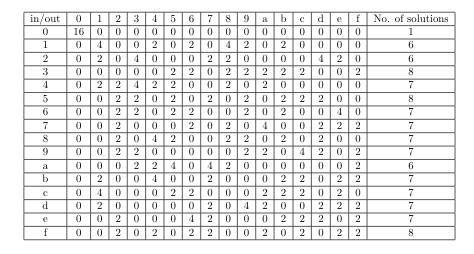
\includegraphics[scale=0.5]{Presentation/sbox.png}
\end{center}
S-box allows 106 out of 256 possible input-output trails. Average non zero values in DDT is 256/106 = 2.415.
\end{frame}

\begin{frame}{Inside-out attack on 2 rounds }  
\begin{center}
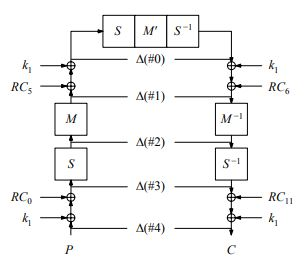
\includegraphics[scale=0.5]{DC.JPG}
\end{center}
\textbf{The differential trail}
\begin{center}
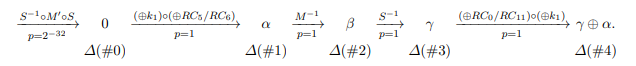
\includegraphics[scale=0.5]{Presentation/test.png}
\end{center}

\end{frame}
\begin{frame}{Inside-out attack on 2 rounds}
\textbf{How the difference propagates:}
\begin{itemize}
    \item \textbf{Key and Round addition:}Difference changes by $\alpha$. $\triangle (\#0)=\alpha\oplus\triangle (\#1)$
    \item \textbf{M or $M^{-1}$:} We can tell with probability 1 the resulting difference
    \item \textbf{Sbox:} Non-linear. Tell how difference propagates based on DDT.
\end{itemize}
    
\end{frame}
\begin{frame}{Inside-out attack on 2 rounds}
\begin{enumerate}
    \item Choose $2^{32}$ plaintexts. We have $\gamma_i\oplus\alpha=P_i\oplus C_i$
    \item By applying the $M'^{−1}$ layer to $\alpha$=$(c0ac || 29b7 || c97c || 50dd)$, we get $\beta$= $(42a3 || 356a || 5d3a || 0fe3)$ with probability 1
    \item From $\beta$ we can get potential values of $\gamma$. This turns out to be 6x8x..x6=$2^{41.38}$.
    Filter out plaintext and ciphertext pairs and expected value to remain is $2^{9.38}$
    \item For every nibble in every remaining $P_i$, we lookup all possible solutions a, b, c, d $\in$ $\{0, 1\}^4$ with a $\oplus$ b = $\gamma_i \xrightarrow{S}$  $\beta = c \oplus d$ There are ($2^{1.27})^ {16} \approx 2^{20.35}$ solutions in average for every $P_i$ for state $(\#3)_i$, which we enumerate by $(\#3)^j_i$: $(\#3)^j_i = P_i \oplus RC0 \oplus k1.$
    \item For each $(\#3)^j_i$ guess $(k_1)^j_i$ and verify if computed cipher is actual ciphertext $C_i$
    \item Full complexity - $2^{32.44}$, memory complexity - $2^{32}$ by storing plaintext, ciphertext and data complexity $2^{32}$ for plaintexts.
\end{enumerate}
    
\end{frame}
\begin{frame}{Inside-out attack on 4 rounds}
\begin{center}
    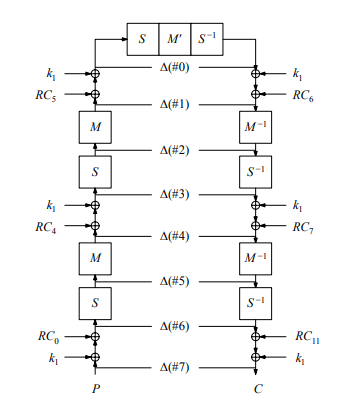
\includegraphics[scale=0.3]{image.png}
    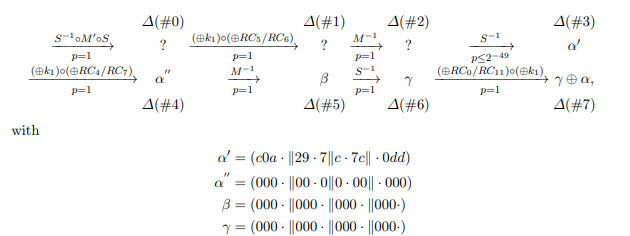
\includegraphics[scale=0.4]{Presentation/myphoto.png}
\end{center}
    
\end{frame}
\begin{frame}{Inside-out attack on 4 rounds}
\textbf{Attack:-}
\begin{itemize}
    \item Choose $2^{48}$ ($P_i,C_i$)pairs
    \item Again derive $\gamma_i = P_i\oplus C_i \oplus \alpha$
    \item Discard pairs where leftmost columns of $\gamma_i$ are not all 0s
    \item Derive possible solutions for a,b,c,d $\in$ $\{0,1\}^{4}$ such that $a\oplus b= \gamma \xrightarrow{S}\beta=c\oplus d$. We estimate $2^{56.08}$ potential values for $(\#6)^j_i$
    \item Derive $(k_1)^j_i$ corresponding to $(\#6)^j_i$ and eliminate false positives by using $(k_1)^j_i$ to encrypt $P_j$ and verify with $C_j$
\end{itemize}
    
\end{frame}
